\documentclass{article}

\usepackage{fullpage}
\usepackage{url}
\usepackage{graphicx}
\usepackage{amsmath}
\usepackage{physics}
\usepackage{mathtools}
\usepackage{bbold}
\usepackage{hyperref}

\hypersetup{
    colorlinks=true,
    linkcolor=blue,
    filecolor=magenta,      
    urlcolor=cyan,
}

\DeclareMathOperator{\erfi}{erfi}
\newcommand{\R}{\ensuremath{\mathbb{R}}}
\newcommand{\C}{\ensuremath{\mathbb{C}}}

\title{General Realtivity Test}
\author{Idan Stark}
\date{\today}

\begin{document}
\maketitle

\section{Question 1}
\subsection{The Helmholtz equation in general coordinates}
In Cartesian coordinates, the Helmholtz equation for the electric field of a monochromatic electromagnetic wave takes the form:
\begin{equation}
    \left(\partial_x^2 + \partial_y^2 + \partial_z^2 + k^2\right)\boldsymbol{E} = 0
\end{equation}
It can be written in Cartesian coordinates as:
\begin{equation}
    \left(\sum_i \partial_i^2 + k^2\right)\boldsymbol{E} = 0
\end{equation}
To move to another coordinate system, all one must do it write the Laplacian $\sum_i \partial_i^2$ in the new set of coordiantes \footnote{I assumed the spatial and temporal coordinates do not mix, since the rest of the question depends only on the spatial coordinates until the covariant derivative.}:
\begin{equation}
    \partial_i^2 = \left(\frac{\partial x'^l}{\partial x^i}\partial_l'\right)^2 = \frac{\partial x'^l}{\partial x^i}\frac{\partial x'^m}{\partial x^i}\partial_l'\partial_m'
\end{equation}
But since
\begin{equation}
    \sum_i \frac{\partial x^i}{\partial x'^l}\frac{\partial x^i}{\partial x'^m} = \gamma'_{lm}
\end{equation}
Then:
\begin{equation}
    \sum_i \partial_i^2 = \gamma'^{lm} \partial_l'\partial_m'
\end{equation}
Which gives (dropping the tags):
\begin{equation}
    \left(\gamma^{ij} \partial_i\partial_j + k^2\right)\boldsymbol{E} = 0
\end{equation}

\subsection{Field in cylindrical coordinates}
The divergence of a general vector $A^i$ in 3D space with the metric $\gamma_{ij}$:
\begin{equation}
    D_i A^i = \frac{1}{\sqrt{\gamma}}\partial_i \sqrt{\gamma}A^i
\end{equation}
Where $\gamma = \det\gamma_{ij}$. In the case of an electric field in cylindrical coordintes with the metric given by
\begin{equation}
    dl^2 = dr^2 + r^2d\phi^2 + dz^2
\end{equation}
With the field only having a component along the $\phi$ direction that depends only on $r, z$:
\begin{equation}
    \boldsymbol{E} = E_\phi(r, z) \hat{\phi}
\end{equation}
We can write:
\begin{equation}
    \gamma_{ij} = diag(1, r^2, 1) \rightarrow \gamma = r^2
\end{equation}
Giving:
\begin{equation}
    \nabla \cdot \boldsymbol{E} = D_i E^i = \frac{1}{r}\partial_i \left(rE^i\right) = \frac{1}{r}\partial_\phi r E^\phi(r, z) = 0
\end{equation}

\subsection{The wave equations}
Starting from the Maxwell equations:
\begin{equation}
\label{eq:maxwell}
    \varepsilon^{ijk}\partial_j E_k = i\omega B^i
    \qquad
    \varepsilon_{ijk}\partial^j B^k = -i\frac{\omega}{c^2} E_i
\end{equation}
We can apply $\varepsilon_{ilm}\partial^l$ to both sides of the first equation. The RHS becomes:
\begin{equation}
    \varepsilon_{ilm}\partial^l i\omega B^i = i\omega \varepsilon_{ilm}\partial^l B^i = - i\omega \varepsilon_{mli}\partial^l B^i = - \frac{\omega^2}{c^2} E_m
\end{equation}
Where we used the symmetries of $\varepsilon_{ijk}$:
\begin{equation}
    \varepsilon_{ilm} = \varepsilon_{lmi} = -\varepsilon_{mli}
\end{equation}
And then plugged in the second equation to get to an expression with the electric field. For the LHS, we can use the fact that (assuming right handed system) $\partial_l \varepsilon_{ijk} = \partial_l \gamma^{-1/2} [ijk] = [ijk]\partial_l \gamma^{-1/2}$ and the property:
\begin{equation}
    [ilm][ijk] = \delta_l^j\delta_m^k - \delta_l^k\delta_m^j
\end{equation}
To get
\begin{equation}
\begin{gathered}
    \varepsilon_{ilm}\partial^l \varepsilon^{ijk}\partial_j E_k = \sqrt{\gamma}[ilm][ijk] \partial^l \frac{1}{\sqrt{\gamma}}\partial_j E_k
    = \\ =
    (\delta_l^j\delta_m^k - \delta_l^k\delta_m^j)\sqrt{\gamma}\partial^l \frac{1}{\sqrt{\gamma}}\partial_j E_k
    = \\ =
    \sqrt{\gamma}\partial^j \frac{1}{\sqrt{\gamma}}\partial_j E_m -
    \sqrt{\gamma}\partial^l \frac{1}{\sqrt{\gamma}}\partial_m E_l
\end{gathered}
\end{equation}
But from the previous section $\partial^l E_l = 0$, so the equation we get is
\begin{equation}
    \sqrt{\gamma}\partial^j \frac{1}{\sqrt{\gamma}}\partial_j E_i  = - \frac{\omega^2}{c^2} E_i
\end{equation}
Or:
\begin{equation}
    \left(\sqrt{\gamma}\partial^j \frac{1}{\sqrt{\gamma}}\partial_j + \frac{\omega^2}{c^2}\right) E_i = 0
\end{equation}
So, for $E_\phi(r,z)$, we get:
\begin{equation}
\begin{gathered}
    \left(r\partial_r \frac{1}{r}\partial_r + \partial^2_z + \frac{\omega^2}{c^2}\right) E_\phi = \\ = 
    \left(\partial_r^2 - \frac{1}{r}\partial_r + \partial^2_z + \frac{\omega^2}{c^2}\right) E_\phi
\end{gathered}
\end{equation}
So the equation becomes
\begin{equation}
    \left(\partial_r^2 - \frac{1}{r}\partial_r + \partial^2_z + \frac{\omega^2}{c^2}\right) E_\phi = 0
\end{equation}

\subsection{Comparing with the scalar field}
The wave equation for a scalar field $A$ is:
\begin{equation}
    D_\mu D^\mu A = \frac{1}{\sqrt{\gamma}}\partial_\mu \sqrt{\gamma}\partial^\mu A = 0
\end{equation}
Where we assumed $g_{00} = 1$, which gives $\sqrt{-g} = \sqrt{\gamma}$. For a scalar field $E(r,z)$ in cylindrical coordinates, this gives:
\begin{equation}
    \frac{1}{r}\partial_\mu r \partial^\mu E = \frac{1}{r}\partial_t r \partial^t E + \frac{1}{r}\partial_r r \partial^r E + \frac{1}{r}\partial_z r \partial^z E = \left(\partial_t^2 + \partial_r^2 + \frac{1}{r}\partial_r +  \partial_z^2 \right) E
\end{equation}
So the equation is:
\begin{equation}
    \left(\partial_t^2 + \partial_r^2 + \frac{1}{r}\partial_r +  \partial_z^2 \right) E = 0
\end{equation}
This result is problematic. The first is that it depends on the order of the derivatives. In the previous section, the derivatives were in opposite order and we got a different result. However, the covariant derivative of a scalar is a vector, and so there is no reason that performing $D^\mu D_\mu$ and $D_\mu D^\mu$ will result in different expressions, even up to a sign. The fact that this is what happened tells me I probably have an arithmetical error.

\subsection{Covariant derivative}
The Christoffel symbols have a symmetry in the last two indices, while the Levi-Civita tensor is anti-symmetric in the same indices, this means that their contraction cancels out and we get:
\begin{equation}
    \varepsilon^{ijk} D_j E_k = \varepsilon^{ijk} (\partial_j E_k - \Gamma^\mu_{jk} A_\mu) = \varepsilon^{ijk} \partial_j E_k - \varepsilon^{ijk} \Gamma^\mu_{jk} A_\mu = \varepsilon^{ijk} \partial_i E_k
\end{equation}
So, the Maxwell equations in equation \ref{eq:maxwell} can be written with the covariant derivative and reach the same result. Furthermore, similarly to the electromagnetic tensor $F^{\mu\nu}$, the covariant derivaive of an antisymmetric 2-tensor is given by:
\begin{equation}
    D_\mu A^{\mu\nu} = \frac{1}{\sqrt{-g}}\partial_\mu \sqrt{-g}A^{\mu\nu}
\end{equation}
So, for the antisymmetric 2-tensor $A^{ij} = \varepsilon^{ijk}E_k$, we get:
\begin{equation}
    D_j \varepsilon^{ijk}E_k = \frac{1}{\sqrt{\gamma}}\partial_\mu \sqrt{\gamma} \varepsilon^{ijk}E_k
\end{equation}
But
\begin{equation}
    \varepsilon^{ijk} = \frac{[ijk]}{\sqrt{\gamma}}
\end{equation}
So:
\begin{equation}
    D_j \varepsilon^{ijk}E_k = \frac{1}{\sqrt{\gamma}}\partial_j [ijk] E_k = \frac{[ijk]}{\sqrt{\gamma}}\partial_j E_k = \varepsilon^{ijk} \partial_j E_k = \partial_j E_k = \varepsilon^{ijk} D_j E_k
\end{equation}

\subsection{Helmholtz equation for a curved space}
For a curved space, we simply use the covariant version of the Maxwell equations. But, according to the relations we just proved, this is the same as using $\partial_j$. The development is then also the same as we did for the specific case of $E_i$ before:
\footnote{Was I supposed to do it in another way before?}
\begin{equation}
    \left(\sqrt{\gamma}\partial^j \frac{1}{\sqrt{\gamma}}\partial_j + \frac{\omega^2}{c^2}\right) E_i = 0
\end{equation}
Where again the curvature is seen in the spatial metric $\gamma$.

\newpage
\section{Question 2}
In this question we explore the metric
\begin{equation}
\label{eq:metric}
    g_{\alpha\beta} = \eta_{\alpha\beta} + A s_{\alpha} s_{\beta}
    \qquad
    A = A(x, y, t - z/c)
    \qquad
    s_\alpha = (1, 0, 0, -1)
\end{equation}

\subsection{Inverse metric}
Let us show that the inverse metric is
\begin{equation}
\label{eq:inverse-metric}
    g^{\alpha\beta} = \eta^{\alpha\beta} - A s^\alpha s^\beta
\end{equation}
where $s^\alpha = (1, 0, 0, 1)$. The inverse metric follows:
\begin{equation}
    g^{\alpha\beta}g_{\beta\gamma} = \delta^\alpha_\gamma
\end{equation}
Pluggin in the metric and the inverse metric, we get:
\begin{equation}
\label{eq:metrics-proof}
\begin{gathered}
    g^{\alpha\beta}g_{\beta\gamma} =
    \left(\eta^{\alpha\beta} - A s^\alpha s^\beta\right)
    \left(\eta_{\beta\gamma} + A s_{\beta} s_{\gamma}\right) = \\ = 
    \eta^{\alpha\beta}\eta_{\beta\gamma}
    + A\left(\eta^{\alpha\beta} s_\beta s_\gamma - \eta_{\beta\gamma}s^{\alpha}s^{\beta}\right)
    - A^2 s^\alpha s^\beta s_\beta s_\gamma
\end{gathered}
\end{equation}
But, from the definition of $s^\alpha$ and $s_\alpha$, we get $s^\beta s_\beta = 1 - 1 = 0$. Additionaly, we can write:
\begin{equation}
    s^{\alpha} = \eta^{\alpha\beta}s_\beta
\end{equation}
And get
\begin{equation}
    \eta^{\alpha\beta}s_\beta s_\gamma = s^\alpha s_\gamma = \eta_{\beta\gamma} s^{\alpha} s^{\beta}
\end{equation}
Which means that the second and third terms in equation \ref{eq:metrics-proof} are zero, giving:
\begin{equation}
    g^{\alpha\beta} g_{\beta\gamma} = \eta^{\alpha\beta}\eta_{\beta_\gamma} = \delta^{\alpha}_{\gamma}
\end{equation}
as required.

\subsection{The nature of $s^\alpha$}
Now, let us show that $s^\alpha = (1, 0, 0, 1)$ follows $s^\alpha = g^{\alpha\beta}s_{\beta}$:
\begin{equation}
    g^{\alpha\beta}s_{\beta} = \left(\eta^{\alpha\beta} - A s^\alpha s^\beta\right)s_\beta = s^\alpha - A s^\alpha s^\beta s_\beta = s^\alpha
\end{equation}
Because, again $s^\beta s_\beta = 0$. In reality, we can find that this specific $s^\alpha$ is the only vector that follows this condition. Starting from $s_\alpha$, we get:
\begin{equation}
    s_\alpha = g_{\alpha\beta}s^{\beta} = \eta_{\alpha\beta} s^\beta + A s_{\alpha} s_{\beta} s^{\beta}
\end{equation}
\begin{equation}
    \left(1 - A s_\beta s^\beta \right)s_\alpha = \eta_{\alpha\beta} s^\beta
\end{equation}
Writing $s^\alpha = (a, b, c, d)$ explicitly, we get:
\begin{equation}
    s_\beta s^\beta = a - d
\end{equation} 
Which gives:
\begin{equation}
    \left(1 - A(a - d)\right)\begin{pmatrix}
        1 \\ 0 \\ 0 \\ -1
    \end{pmatrix} = \begin{pmatrix}
        a \\ -b \\ -c \\ -d
    \end{pmatrix}
\end{equation}
This gives $b = c = 0$ and after substrating the first and last equations, $a = d = 1$ for all $A$. So $s^{\alpha} = (1, 0, 0, 1)$.
\newline
The reason for this specific $s^\alpha$ to work is that $A$ does not depends on $t$ or $z$ directly, but rather on the expression $t - z/c$ that is zero only on the line defined by the null vector $s_\alpha$. This means that the change of $A$ along the perpendicular line $s^\alpha$ vanishes. Marking $w = t - z/c$, we get:
\begin{equation}
    s^\alpha \partial_\alpha A = (1,0,0,-1)\cdot\left(\frac{1}{c}\partial_t, -\vec{\nabla}\right)A = \frac{1}{c}\partial_t A + \partial_z A = \left(\frac{\partial w}{c\partial t} + \frac{\partial w}{\partial z}\right)\frac{\partial A}{\partial w} = 0
\end{equation}

\subsection{Christoffel symbols}
First, let us notice that:
\begin{equation}
    \partial_\mu g_{\alpha\beta} = \partial_\mu \left(\eta_{\alpha\beta} + A s_{\alpha} s_{\beta}\right) = s_\alpha s_\beta \partial_\mu A 
\end{equation}
Now, using the formula for Christoffel symbols:
\begin{equation}
\begin{gathered}
    \Gamma^\mu_{\alpha\beta} = \frac{1}{2}g^{\mu\nu}\left(\partial_{\alpha}g_{\nu\beta} + \partial_{\beta}g_{\nu\alpha} - \partial_{\nu}g_{\alpha\beta}\right) = \\ = \frac{1}{2}\left(\eta^{\mu\nu} - A s^\mu s^\nu\right)
    \left(
        s_\nu s_\beta \partial_\alpha A 
        + s_\nu s_\alpha \partial_\beta A 
        - s_\alpha s_\beta \partial_\nu A 
    \right) = \\ = \frac{1}{2}\eta^{\mu\nu}
    \left(
        s_\nu s_\beta \partial_\alpha A 
        + s_\nu s_\alpha \partial_\beta A 
        - s_\alpha s_\beta \partial_\nu A 
    \right) - \frac{1}{2}A\left(
        s^\mu s^\nu s_\nu s_\beta \partial_\alpha A 
        + s^\mu s^\nu s_\nu s_\alpha \partial_\beta A 
        -s^\mu s_\alpha s_\beta s^\nu \partial_\nu A 
    \right)
\end{gathered}
\end{equation}
But since both $s^\nu s_\nu = 0$ and $s^\nu \partial_\nu A = 0$, the second paranthesses vanish and we get:
\begin{equation}
    \Gamma^\mu_{\alpha\beta} = \frac{1}{2}\eta^{\mu\nu}
    \left(
        s_\nu s_\beta \partial_\alpha A 
        + s_\nu s_\alpha \partial_\beta A 
        - s_\alpha s_\beta \partial_\nu A 
    \right)
\end{equation}
Moving $\eta^{\mu\nu}$ inside and using $\eta^{\mu\nu}s_\nu = s^\mu$ and
\begin{equation}
    \partial^\mu A = g^{\mu\nu}\partial_\nu A = (\eta^{\mu\nu} - A s^\mu s^\nu)\partial_\nu A = \eta^{\mu\nu} \partial_\nu A - A s^\mu s^\nu \partial_\nu A = \eta^{\mu\nu} \partial_\nu A
\end{equation}
We can write this as:
\begin{equation}
\label{eq:christoffel-final}
    \Gamma^\mu_{\alpha\beta} = \frac{1}{2}
    \left(
        s^\mu s_\beta \partial_\alpha A 
        + s^\mu s_\alpha \partial_\beta A 
        - s_\alpha s_\beta \partial^\mu A 
    \right)
\end{equation}

\subsection{Important property of $\Gamma^\mu_{\alpha\beta}$}
Contracting the first and third indices in the equation \ref{eq:christoffel-final}, we get:
\begin{equation}
\begin{gathered}
    \Gamma^\beta_{\alpha\beta} = \frac{1}{2}
    \left(
        s^\beta s_\beta \partial_\alpha A 
        + s^\beta s_\alpha \partial_\beta A 
        - s_\alpha s_\beta \partial^\beta A 
    \right) = \frac{1}{2}
    \left(
        s^\beta s_\beta \partial_\alpha A 
        + s_\alpha s^\beta \partial_\beta A 
        - s_\alpha s^\beta \partial_\beta A 
    \right) = 0
\end{gathered}
\end{equation}
Where again in the first term we used $s^\beta s_\beta = 0$ and the last two terms we used $s^\beta \partial_\beta = 0$.

\subsection{Non-linear terms in the Ricci tensor}
The Ricci tensor can be calculated then using the Christoffel symbols:
\begin{equation}
    R_{\mu\nu} =
    \partial_\alpha \Gamma^\alpha_{\mu\nu}
    - \partial_\nu \Gamma^\alpha_{\mu\alpha}
    + \Gamma^\sigma_{\mu\nu} \Gamma^\alpha_{\sigma\alpha}
    + \Gamma^\sigma_{\mu\alpha} \Gamma^\alpha_{\sigma\nu}
\end{equation}
It is obvious from the last section that the third term $\Gamma^\sigma_{\mu\nu} \Gamma^\alpha_{\sigma\alpha}$ vanishes. The last term gives:
\begin{equation}
    \Gamma^\sigma_{\mu\alpha} \Gamma^\alpha_{\sigma\nu} = \frac{1}{4}
    \left(
        s^\sigma s_\alpha \partial_\mu A 
        + s^\sigma s_\mu \partial_\alpha A 
        - s_\mu s_\alpha \partial^\sigma A 
    \right)
    \left(
        s^\alpha s_\nu \partial_\sigma A 
        + s^\alpha s_\sigma \partial_\nu A 
        - s_\sigma s_\nu \partial^\alpha A 
    \right)
\end{equation}
On one hand, each of the terms in the left paranthesses includes either $s^\sigma$ or $s_\alpha$. On the other hand. each of the terms on the right paranthesses includes a $\sigma$ factor, either $s_\sigma$ or $\partial_\sigma A$ that will vanish with the terms in the first paranthesses that include $s^\sigma$, and an $\alpha$ factor, either $s^\alpha$ or $\partial_\alpha$ factor that will vanish the terms that includes $s_\alpha$ on the left. Thus, all terms vanish and we get:
\begin{equation}
    \Gamma^\sigma_{\mu\alpha} \Gamma^\alpha_{\sigma\nu} = 0
\end{equation}

\subsection{The Ricci tensor}
We can thus write the Ricci tensor as:
\begin{equation}
    R_{\mu\nu} =
    \partial_\alpha \Gamma^\alpha_{\mu\nu}
    - \partial_\nu \Gamma^\alpha_{\mu\alpha}
\end{equation}
But the second term again vanishes, from section 2.4:
\begin{equation}
\begin{gathered}
    R_{\mu\nu} = 
    \partial_\alpha \Gamma^\alpha_{\mu\nu}
    =
    \frac{1}{2}
    \partial_\alpha \left(
        s^\alpha s_\nu \partial_\mu A 
        + s^\alpha s_\mu \partial_\nu A 
        - s_\mu s_\nu \partial^\alpha A 
    \right) = \\ =
    \frac{1}{2}
    \left(
        s^\alpha s_\nu \partial_\mu \partial_\alpha A 
        + s^\alpha s_\mu \partial_\nu \partial_\alpha  A 
        - s_\mu s_\nu \partial_\alpha \partial^\alpha A 
    \right) = \\ =
    -\frac{1}{2} s_\mu s_\nu \partial_\alpha \partial^\alpha A 
\end{gathered}
\end{equation}
But, since from the definition of $A$, $\frac{1}{c}\partial_t A = \partial_z A$, we get:
\begin{equation}
\begin{gathered}
    \partial_\alpha \partial^\alpha A = \left(
        \frac{1}{c^2}\partial_t \partial^t - \partial_x \partial^x - \partial_y \partial^y - \partial_z \partial^z
    \right) A = \\ =
     \left(
        \frac{1}{c}\partial_t \partial^z - \partial_x \partial^x - \partial_y \partial^y - \frac{1}{c}\partial_z \partial^t
    \right) A = - \left(\partial_x^2 + \partial_y^2\right) A
\end{gathered}
\end{equation}
So:
\begin{equation}
    R_{\mu\nu} = \frac{1}{2}s_\mu s_\nu \left(\partial_x^2 + \partial_y^2\right) A
\end{equation}

\subsection{The Energy-Momentum Tensor}
We can now use Einstein's equations to find $T_{\mu\nu}$:
\begin{equation}
    R_{\mu\nu} - \frac{1}{2}R g_{\mu\nu} = \frac{8\pi G}{c^4}T_{\mu\nu}
\end{equation}
First let us find the scalar curvature:
\begin{equation}
    R = g^{\mu\nu} R_{\mu\nu} =
    \left(\eta^{\mu\nu} - A s^\mu s^\nu\right)\frac{1}{2}s_\mu s_\nu \left(\partial_x^2 + \partial_y^2\right) A = \left(s_\nu s^\nu - A s_\mu s^\mu s_\nu s^\nu\right)\frac{1}{2} \left(\partial_x^2 + \partial_y^2\right) A = 0
\end{equation}
So:
\begin{equation}
\label{eq:energy-momentum}
    T^{\mu\nu} = \frac{c^4}{8 \pi G} R^{\mu\nu} = \frac{c^4}{16 \pi G}s^\mu s^\nu \left(\partial_x^2 + \partial_y^2\right) A
\end{equation}

\subsection{Superposition}
Let us now look at the total energy momentum tensor from two such systems:
\begin{equation}
    T_{1}^{\mu\nu} = \frac{c^4}{16 \pi G}s^\mu s^\nu \left(\partial_x^2 + \partial_y^2\right) A_1
    \qquad
    T_{1}^{\mu\nu} = \frac{c^4}{16 \pi G}s^\mu s^\nu \left(\partial_x^2 + \partial_y^2\right) A_2
\end{equation}
And the total:
\begin{equation}
    T^{\mu\nu} = \frac{c^4}{16 \pi G}s^\mu s^\nu \left(\partial_x^2 + \partial_y^2\right) (A_1 + A_2)
\end{equation}
This follows the same structure, with a new function $A = A_1 + A_2$. The resulting metric will then be the same metric as in equation \ref{eq:metric}, with this new $A$.
\newline
This is the key property of this system: Einstein's equations are not usually linear, so they do not observe superposition. But by limiting the metric to be only the Minkowski metric $\eta_{\mu\nu}$ plus and that is constant along the null geodesics, it reduces the Einstein equations to a linear form and thus allow superposition.

\subsection{Effect on test particles}
The infinitisimal action of a particle is given by: 
\begin{equation}
\begin{gathered}
    ds^2 = g_{\mu\nu}dx^\mu dx^\nu = \left(\eta_{\mu\nu} + A s_\mu s_\nu\right) dx^\mu dx^\nu = \\ =
    c^2dt^2 - dx^2 - dy^2 - dz^2 + Ac^2dt^2 + A dz^2 - 2Acdtdz
    = \\ =
    \left[(1 + A)c^2 - \dot{x}^2 - \dot{y}^2 - (1 - A)\dot{z}^2 - 2Ac\dot{z}\right] dt^2
\end{gathered}
\end{equation}
Now, let us write $A = \frac{2\varphi}{c^2}$ and neglect all instances $\beta^i = \dot{x}^i/c$:
\begin{equation}
\begin{gathered}
    ds^2 = 
    \left[\left(1 + \frac{2\varphi}{c^2}\right)c^2 - \dot{x}^2 - \dot{y}^2 - \left(1 - \frac{2\varphi}{c^2}\right)\dot{z}^2 - 2\frac{2\varphi}{c^2}c\dot{z}\right] dt^2
    = \\ =
    \left[\left(1 + \frac{2\varphi}{c^2}\right)c^2 - \dot{x}^2 - \dot{y}^2 - \dot{z}^2\right] dt^2
    = \\ =
    \left(1 + \frac{2\varphi}{c^2}\right)c^2 dt^2 - dx^2 - dy^2 - dz^2
\end{gathered}
\end{equation}
This is the infinitisimal action of the Newtonian limit, given by the condition
\begin{equation}
    g_{00} = 1 + \frac{2\varphi}{c^2}
\end{equation}
In other words, for non-relativistic particles, the addition of $s_\mu s_\nu A$ to the Minkowski metric is akin to the addition of a gravitational potential $\varphi = \frac{1}{2}c^2A$.

\subsection{Back to the Energy Momentum Tensor}
The Energy-Momentum Tensor of a fluid is given by:
\begin{equation}
    T^{\mu\nu} = (\varepsilon + p)u^\mu v^\mu - pg^{\mu\nu}
\end{equation}
Where $\varepsilon$ is the energy density and $p$ is the pressure. Comparing this to the energy-momentum tensor we found in equation \ref{eq:energy-momentum}, we get:
\begin{equation}
\label{eq:em-tensors}
    (\varepsilon + p)u^\mu u^\nu - pg^{\mu\nu} = \frac{c^4}{16 \pi G}s^\mu s^\nu \left(\partial_x^2 + \partial_y^2\right) A
\end{equation}
Contracting $\mu$ with $\nu$, and using:
\begin{equation}
    g_{\mu\nu}u^\mu u^\nu = 1
    \qquad
    g_{\mu\nu}g^{\mu\nu} = 4
    \qquad
    g_{\mu\nu}s^\mu s^\nu = s_\nu s^\nu = 0
\end{equation}
We get:
\begin{equation}
    (\varepsilon + p) - 4p = 0
\end{equation}
\begin{equation}
    p = \frac{\varepsilon}{3}
\end{equation}

\subsection{General Fluid from lab frame}
Given a fluid in Minkowski space that moves with the four-velocity $u^\mu = (\cosh\xi, 0, 0, \sinh \xi)$, with $v = c\tanh\xi$, the ordinary velocity. Let $\varepsilon_0$ be the laboratory energy density, while the energy momentum tensor can be written as:
\begin{equation}
    T^{\mu\nu} = (\varepsilon + p)u^\mu u^\nu - p\eta^{\mu\nu}
\end{equation}
with the co-moving energy density $\varepsilon$. So, to find $\varepsilon$ in terms of $\varepsilon_0$, let us use Lorentz transformation from the lab frame to the co-moving frame $u^\mu = (1, 0, 0, 0)$. The Lorentz transformation to this frame corresponds to $\beta = -v/c = -\tanh \xi$ and $\gamma = (1 - \beta^2)^{-1/2} = \cosh \xi$ and results, not surprisingly, in the diagonal energy-momentum tesnor:
\begin{equation}
    T'^{\mu\nu} = diag(\varepsilon, p, p, p)
\end{equation}
And thus the energy density, $\varepsilon$ is related to the lab-frame energy density based on the regualr density contraction:
\footnote{I'm pretty sure I didn't get what I was supposed to do here. This seems trivial.}
\begin{equation}
    \varepsilon = \gamma^{-1}\varepsilon_0 = \frac{\varepsilon_0}{\cosh\xi}
\end{equation}

\subsection{Conclusion}
Before I list my errors that I didn't have time to correct, I want to note that I do understand the result of this question:  In this interpertation, $\epsilon_0$ is the "charge density" for the potential $\phi$ related to $A$ as described before, creating the flow described by the velocity $\beta = \tanh \xi = 1$.
\newline
Now, for the errors. From the structure of the energy-momentum tensor for a fluid, I get that $\cosh \xi = \sinh \xi$ which fits $\beta = 1$ for massless fluid. But, I also get $p = 0$. This is an issue since on the one hand $\varepsilon = 3p$ but on the other $\varepsilon \ne 0$.
\newline
I think maybe I was wrong to write $u_\mu u^\mu = 1$, since this only true for the Minkowski metric, but I don't have time to recalcualte it.
\newline
That being said, the probable next step is to find the error, which will probably result in $p = 0$, and the above interpertation arising from it.

\newpage
\section{Question 4}
In this section we look at Mach conjecture, starting from an empty universe with the first Friedman equation:
\begin{equation}
\label{eq:friedmann-1}
    H^2 + \frac{Kc^2}{a^2} = \frac{8\pi G}{3}\rho
\end{equation}
where $H = \dot{a}/a$ is the Hubble parameter, $\rho$ is the mass density, and $K \in \{-1, 0, +1\}$ characterizes the spatial curvature.

\subsection{Possible curvatures}
Let us assume the the universe is both empty $\rho = 0$ and flat $K = 0$. This gives
\begin{equation}
    \frac{\dot{a}^2}{a^2} = 0
\end{equation}
\begin{equation}
    \dot{a} = 0
\end{equation}
So, an empty flat universe does not expand. On the other hand, for a non-flat universe $K = \pm 1$:
\begin{equation}
    \frac{\dot{a}^2}{a^2} \pm \frac{c^2}{a^2} = 0
\end{equation}
\begin{equation}
    \dot{a} = \pm c
\end{equation}
So, a spherical universe $K = 1$ will collapse with constant speed $-c$, while a hyperbolic universe $K = -1$ will expand with constant speed $c$. The conclusion is, that if we start from $a = 0$, the only universe that can exist is the hyperbolic one with $K = -1$, with the scale factor changing linearly in cosmological time:
\begin{equation}
    a(t) = ct
\end{equation}

\subsection{The metric}
According to the cosmological principle, the metric for this space must be homogenous and isotropic. According to the theorem by Robertson and Walker, the only metric that abide by noth those things is the FLRW metric. For a negatively curved space with curvature $K$, it is given by the line element
\begin{equation}
    ds^2 = c^2dt^2 - a^2\left(
        d\chi^2 + \sqrt{|K|}^{-2}\sinh(\sqrt{|K|}\chi)^2d\Omega^2
    \right)
\end{equation}
Plugging in $K = -1$, we get:
\begin{equation}
    ds^2 = c^2dt^2 - a^2\left(
        d\chi^2 + \sinh^2 \chi d\Omega^2
    \right)
\end{equation}

\subsection{Transformation to Minkowski space-time}
Assinging the scale factor into the metric gives:
\begin{equation}
    ds^2 = c^2dt^2 - c^2t^2\left(
        d\chi^2 + \sinh^2 \chi d\Omega^2
    \right)
\end{equation}
Let us define the transformation:
\begin{equation}
    r_m = ct \sinh \chi
    \qquad
    ct_m = ct \cosh \chi
\end{equation}
And the opposite transformation:
\begin{equation}
    c^2t^2 = c^2t_m^2 - r_m^2
    \qquad
    \chi = \tanh^{-1}\left(\frac{r_m}{ct_m}\right)
\end{equation}
The differntials:
\begin{equation}
    cdt = \frac{t_m dt_m - r_m dr_m}{ct}
    \qquad
    d\chi = \frac{t_m dr_m - r_m dt_m}{(ct)^2}
\end{equation}
Pluggin these in the line element, and using $ct\sinh\chi = r_m$:
\begin{equation}
\begin{gathered}
    ds^2 = \left(\frac{c^2t_m dt_m - r_m dr_m}{ct}\right)^2 - c^2t^2\left(\frac{ct_m dr_m - cr_m dt_m}{(ct)^2}\right)^2 - r_m^2 d\Omega^2 = \\ =
    \frac{t_m^2 dt_m^2 - t_m r_m dt_m dr_m + r_m^2 dr_m^2}{(ct)^2} - \frac{r_m^2 dt_m^2 - t_m r_m dt_m dr_m + t_m^2 dr_m^2}{(ct)^2} - r_m^2 d\Omega^2 = \\ =
    \frac{c^2t_m^2 - r_m^2}{(ct)^2}c^2dt_m^2 - \frac{r_m^2 - c^2t_m^2}{(ct)^2}dr_m^2 - r_m^2 d\Omega^2 = \\ =
    c^2dt_m^2 - dr_m^2 - r_m^2 d\Omega^2 
\end{gathered}
\end{equation}
So, under this transformation we got a Minkowski space-time.

\subsection{The Riemann Tensor}
Since this space is empty, the Ricci Tensor is zero. However, this is not true for the Riemann tensor. In general, the Riemann tensor includes information that the Ricci tensor doesn't include, and therefore even if Einstein's equations result in the Ricci tensor being zero, the Riemann tensor doesn't generally vanish.
\newline
The Riemann tensor is defines by the change in a vector when it's being parallelly transported along a closed loop. The first two indices are for the new vector and the old vector, while the last two indices are for the two directions of the parallel transport, expressed in the definition using covariant derivatives. The Ricci tensor is then the trace along the first and third index, giving the sum of changes of such vectors when parallelly transported along such loops, where the vector is parallel to one of the directions in the loop. Since, unlike the Ricci tensor, the Riemann tensor includes the change along a generic loop, it includes information about the curvature of spacetime that doesn't result from the energy-momentum tensor in Einstein's equations, but by the intrensic property of the universe as a Riemannian manifold.
\newline
For the FLRW metric that we saw with a scale factor linear in time, we can calculate the Riemann tensor in the new coordinates, and then use the tensor transformation to the old coordinates. However, the Riemann tensor in the new coordinates is simply the Riemann tensor of Minkowski space-time, which is zero.
\newline
In conclusion, even thuogh in general the Riemann tensor of an empty universe can be non-zero, following the cosmological principle for a universe with a start (a time $t = 0$ where $a = 0$), it must vanish identically.
\newline
This is a realization of Mach's principle. The fact that the universe is empty, meaning that there is not even background mass, identifies all of its curvature DOF, not just those that are defined by Einstein's equations.

\subsection{The region occupied by the expanding space}
This space expands at a constant speed $c$. The area it will take in the Minkowski coordinates $t_m, r_m$ is given by all values of $\chi$ for a given $t$. Using the inverse transformation, we can see that the two conditions are:
\begin{equation}
\label{eq:minkowski-conditions}
    (i) \ c^2t_m^2 - r_m^2 < c^2t^2
    \qquad
    (ii) \ \left|\frac{r_m}{ct_m}\right| < 1
\end{equation}
Condition $(i)$ defines the expansion of the universe with cosmological time, while condition $(i)$ limits it to the spacelike region of the Minkowski space-time. The total space can be seen in figure \ref{fig:minkowski-spacetime}.
\begin{figure}[h]
    \centering
    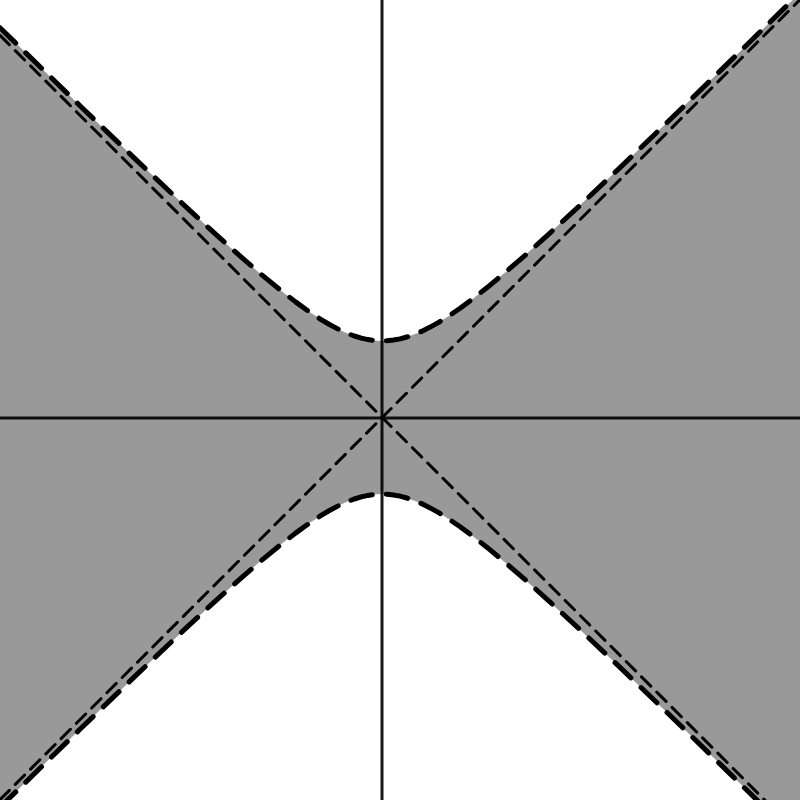
\includegraphics[width=0.25\textwidth]{desmos-graph (15).png}
    \hspace{4mm}
    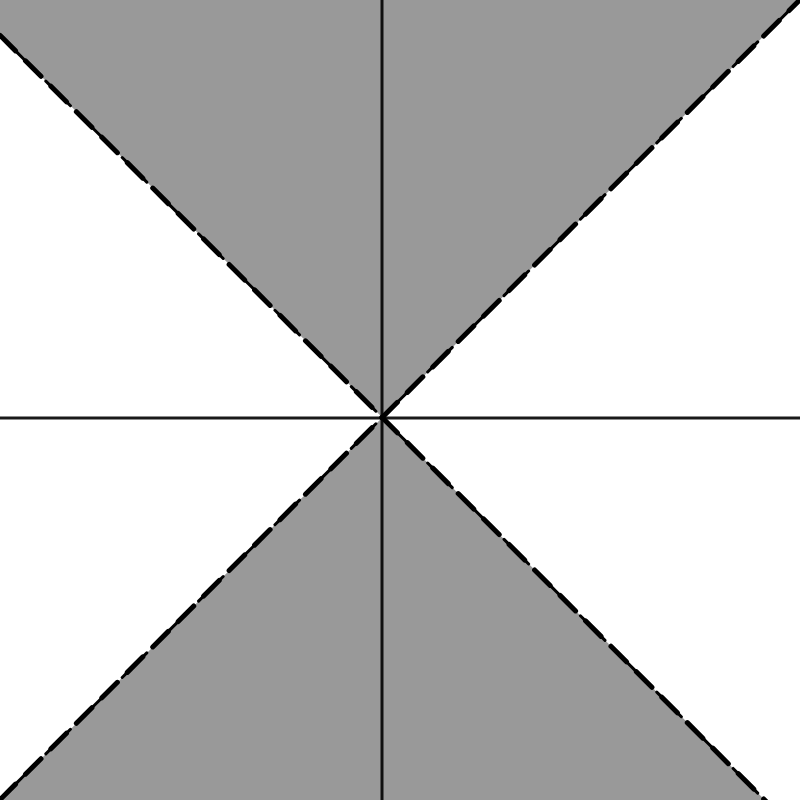
\includegraphics[width=0.25\textwidth]{desmos-graph (16).png}
    \hspace{4mm}
    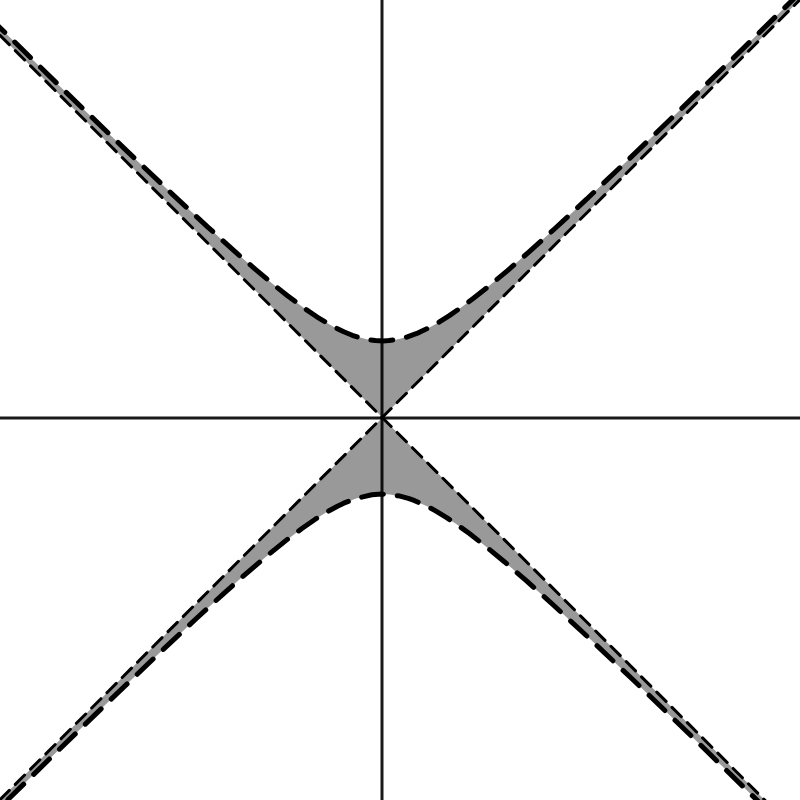
\includegraphics[width=0.25\textwidth]{desmos-graph (17).png}
    \caption{The region of Minkowski space $(t_m , r_m)$ responding to the conditions in equation \ref{eq:minkowski-conditions}. The horizontal axis corresponds to $r_m$ and the vertical axis corresponds to $ct_m$. The narrow dashes lines correspond to $r_m = \pm ct_m$. From left to right: The region reprenting condition $(i)$, the region reprenting condition $(ii)$, and the region reprenting both conditions. The region reprenting both conditions on the rightmost figure is the region of space-time occupied by the exapnding space at time $t$.}
    \label{fig:minkowski-spacetime}
\end{figure}
\newline
The trajectories of comoving points will go along changes in cosmological time, i.e. the lines with constant $\chi$:
\begin{equation}
\label{eq:comoving-points}
    r_m = \tanh\chi ct_m
\end{equation}
These are straight lines originating from the origin. They represent stationary points in the comoving coordinates frame, and thus represent "static" objects in that frame. They are constantly moving away from eachother as the universe expands, starting from $t = 0$ and constantly expanding. These trajectories can be seen in figure \ref{fig:comoving-trajectories}.
\begin{figure}[h]
    \centering
    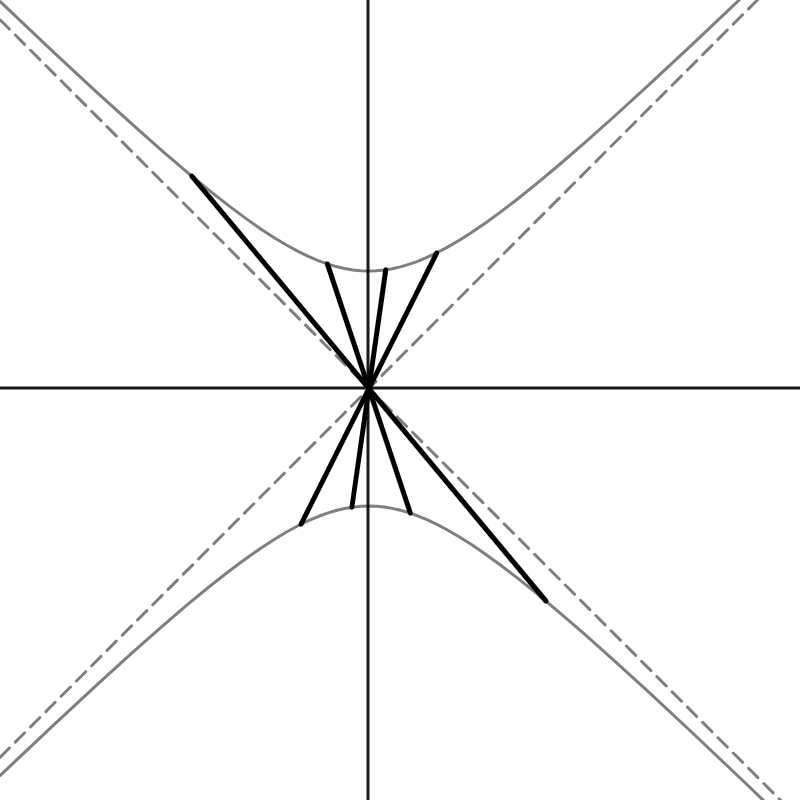
\includegraphics[width=0.25\textwidth]{desmos-graph (18).png}
    \caption{Trajectories in Minkowski space-time of four comoving points.}
    \label{fig:comoving-trajectories}
\end{figure}

\subsection{Velocities and proper time of comoving points}
From equation \ref{eq:comoving-points}, it's obvious that their velocities in Minkowski-spacetime:
\begin{equation}
    \frac{dr_m}{dt_m} = c\tanh \chi
\end{equation}
Their proper time is then (using $d\Omega = 0$):
\begin{equation}
    c^2d\tau^2 = ds^2 = c^2dt_m^2 - dr_m^2 - r_m^2 d\Omega^2 = \left(1 - \tanh^2 \chi\right)c^2dt_m^2
\end{equation}
But along the comoving tranjectory $d\chi = 0$:
\begin{equation}
    cdt_m = cd(t \cosh \chi) = \cosh\chi cdt
\end{equation}
And since
\begin{equation}
    1 - \tanh^2 \chi = 1 - \frac{\sinh^2 \chi}{\cosh^2 \chi} = \cosh^{-2}\chi
\end{equation}
We get:
\begin{equation}
    c^2 d\tau^2 = \left(1 - \tanh^2 \chi\right)\cosh^2 \chi c^2 dt^2 = c^2 dt^2
\end{equation}
And so the cosmological time $t$ is the proper time of the comoving points, as expected. This is a general result stemming from their definition. A comoving point is spatially static in the comoving frame. So, their proper time is the proer time of the comoving frame, which is by definition the cosmological time.

\subsection{The curvature of the expanding space}
The expanding empty space is curved while space-time is flat. This can be seen from the same-cosmological-time surfaces
\begin{equation}
    c^2t_m^2 - r_m^2 = const
\end{equation}
Which are hyperbolic in nature. They describe space at a given point in time. In a sense, we can think of space as expanding "non-uniformally". Not in the 3D spatial sense, since it is homogenous and isotropic, but in a 4D sense, some parts of space "move faster" then other parts, creating these hyperbolic planes.

\subsection{Cosmological Hoirzon}
Let us look for the cosmological horizon. For this, let us take a lightlike object $c^2dt_m^2 = dr_m^2$ and calcualte the distance it will pass. The time $t = 0$ is defined in the Minkowski space-time along the lines $r_m = \pm ct_m$. However, starting from $t = 0, \chi = 0$ means starting from the origin, then for that specific trajectory there is no horizon - i.e. a static horizon at infinity:
\begin{equation}
    \eta = \int_0^t \frac{dt'}{a(t')} = \int_0^t \frac{dt'}{ct'} = \infty
\end{equation}

\subsection{Gibbons-Hawking temperature}
Not only is the horizon at infinity, it also does not radiate and an observer will not feel the Gibbons-Hawking temperature. The radiation came from conservation of energy around the horizon, but since the horizon is at infinity, i.e. no comoving observers reach it, it does not radiate.

\end{document}